\subsubsection{UCA 1 - Accesso all'applicazione}%kite level

\begin{figure}[h]
  \centering
    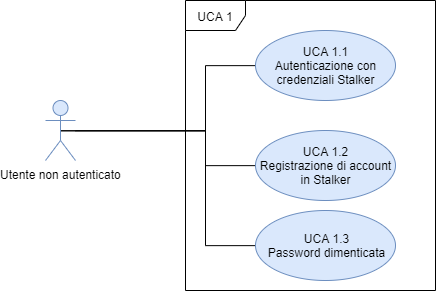
\includegraphics[scale=0.8]{sezioni/UseCase/Immagini/UCA1.png}
  \caption{UCA 1 -  Accesso all'applicazione}
\end{figure}

\begin{itemize}
\item \textbf{Attori primari:} Utente non autenticato;
\item \textbf{Precondizione:} L'utente non è autenticato;
\item \textbf{Postcondizione:} L'utente viene autenticato all'interno del sistema;
\item \textbf{Scenario principale:} L'utente non identificato può scegliere se registrarsi nel sistema oppure, se possiede già un account, accedere all'applicazione; %cosa potrebbe fare l'utente con il UC, descrizione
%\item \textbf{Estensioni:}
\item \textbf{Flusso di eventi:}
    \begin{enumerate}
        \item UCA 1.1 - Autenticazione con credenziali Stalker;
        \item UCA 1.2 - Registrazione di account in Stalker.
    \end{enumerate}

\end{itemize}

\subsubsection{UCA 1.1 - Autenticazione con credenziali Stalker}%sea level

\begin{figure}[h]

  \centering
    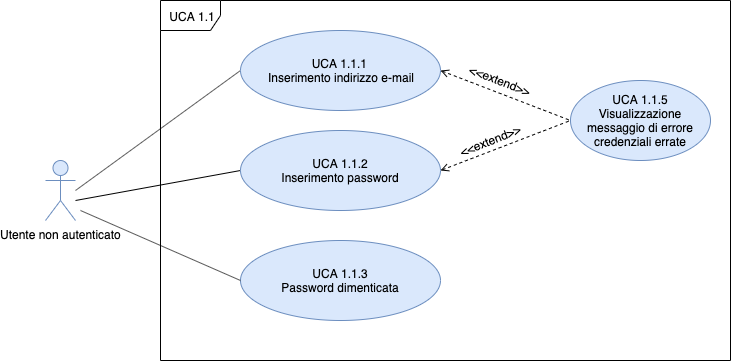
\includegraphics[scale=0.4]{sezioni/UseCase/Immagini/Login.png}
  \caption{UCA 1.1 - Autenticazione con credenziali Stalker}
\end{figure}

\begin{itemize}
\item \textbf{Attori primari:} Utente non autenticato;
%\item \textbf{Attori secondari:}%opzionale
\item \textbf{Precondizione:} L'utente non è autenticato;
\item \textbf{Postcondizione:} L'utente viene autenticato all'interno del sistema e può accedere all'applicazione;
\item \textbf{Scenario principale:} L'utente non autenticato inserisce l'indirizzo e-mail e la password per autenticarsi attraverso la dashboard\ap{G} iniziale%cosa potrebbe fare l'utente con il UC, descrizione
\item \textbf{Flusso di eventi:} %elenco puntato
  \begin{enumerate}
        \item UCA 1.1.1 - Inserimento indirizzo e-mail;
        \item UCA 1.1.2 - Inserimento password;
        \item UCA 1.1.3 - Password dimenticata;
    \end{enumerate}
\item \textbf{Estensioni:}
	\begin{itemize}
		\item UCA 1.1.4 - Visualizzazione messaggio di errore credenziali errate.
	\end{itemize}
%\item \textbf{Inclusioni:}
\end{itemize}

\subsubsection{UCA 1.1.1 - Inserimento indirizzo e-mail}%fish level
\begin{itemize}
\item \textbf{Attori primari:}  Utente non autenticato;
%\item \textbf{Attori secondari:}%opzionale
\item \textbf{Precondizione:}  L'utente non è autenticato;
\item \textbf{Postcondizione:}  L'utente ha inserito il proprio indirizzo e-mail.
\end{itemize}

\subsubsection{UCA 1.1.2 - Inserimento password}%fish level
\begin{itemize}
\item \textbf{Attori primari:} Utente non autenticato;
%\item \textbf{Attori secondari:}%opzionale
\item \textbf{Precondizione:} L'utente non è autenticato;
\item \textbf{Postcondizione:} L'utente ha inserito la propria password.
\end{itemize}

%\subsubsection{UCA 1.1.3 - Pulsante accedi}%fish level
%\begin{itemize}
%\item \textbf{Attori primari:} Utente non autenticato
%\item \textbf{Attori secondari:}%opzionale
%\item \textbf{Precondizione:} L'utente non autenticato
%\item \textbf{Postcondizione:} L'utente ha fatto richiesta per essere autenticato dal sistema 
%\end{itemize}

\subsubsection{UCA 1.1.3 - Password dimenticata}%fish level
\begin{itemize}
\item \textbf{Attori primari:} Utente non autenticato;
%\item \textbf{Attori secondari:}%opzionale
\item \textbf{Precondizione:}  L'utente non è autenticato;
\item \textbf{Postcondizione:} L'utente ha fatto richiesta per avviare la procedura di password dimenticata.
\end{itemize}

\subsubsection{UCA 1.1.4 - Visualizzazione messaggio di errore credenziali errate}%fish level
\begin{itemize}
\item \textbf{Attori primari:} Utente non autenticato;
%\item \textbf{Attori secondari:}%opzionale
\item \textbf{Precondizione:}  L'utente non è autenticato;
\item \textbf{Postcondizione:} L'utente visualizza un messaggio di errore a causa delle credenziali inserite in modo errato.
\end{itemize}

\subsubsection{UCA 1.2 - Registrazione di account in Stalker}%sea level

\begin{figure}[h]
  \centering
    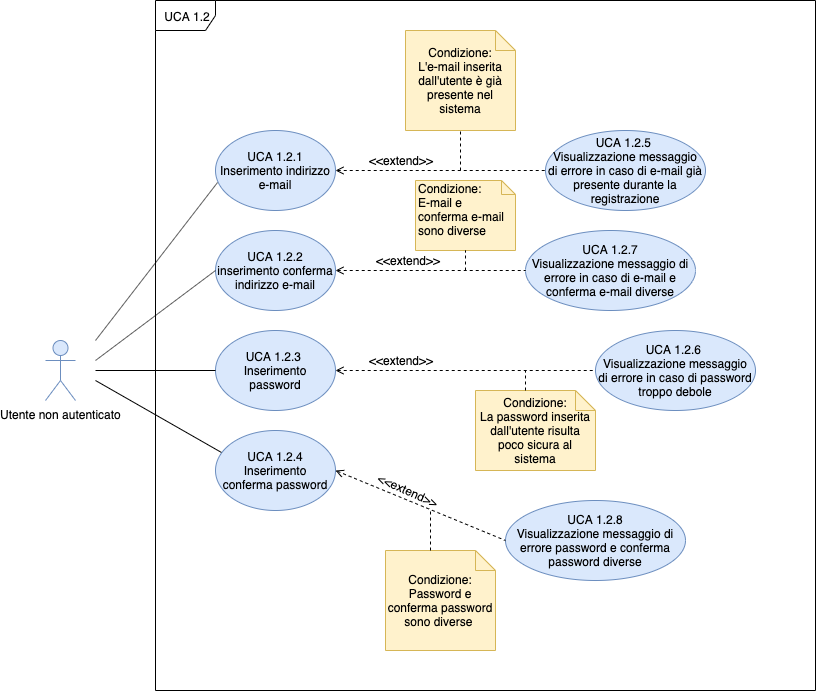
\includegraphics[scale=0.5]{sezioni/UseCase/Immagini/Registrazione.png}
  \caption{UCA 1 -  Registrazione di account in Stalker}
\end{figure}

\begin{itemize}
\item \textbf{Attori primari:} Utente non autenticato;
%\item \textbf{Attori secondari:}%opzionale
\item \textbf{Precondizione:} L'utente non é ancora registrato nel sistema;
\item \textbf{Postcondizione:} L'utente si è registrato e può accedere al sistema;
\item \textbf{Scenario principale:} L'utente non registrato compila il modulo di registrazione al fine di poter accedere al sistema;%cosa potrebbe fare l'utente con il UC, descrizione
\item \textbf{Flusso di eventi:} %elenco puntato
  \begin{enumerate}
        \item UCA 1.2.1 - Inserimento indirizzo e-mail;
        \item UCA 1.2.2 - Inserimento password;
        \item UCA 1.2.3 - Inserimento conferma password;
    \end{enumerate}
\item \textbf{Estensioni:}
	\begin{itemize}
		\item UCA 7.1.1 - Visualizzazione messaggio di errore in caso di e-mail già presente durante la registrazione;
		\item UCA 7.1.2 - Visualizzazione messaggio di errore in caso di password troppo debole;
		\item UCA 7.1.3 - Visualizzazione messaggio di errore in caso di password e conferma password diverse. 
	\end{itemize}
%\item \textbf{Inclusioni:}
\end{itemize}

\subsubsection{UC 1.2.1 - Inserimento indirizzo e-mail}%fish level

\begin{itemize}
\item \textbf{Attori primari:} Utente non autenticato;
%\item \textbf{Attori secondari:}%opzionale
\item \textbf{Precondizione:} L'utente non è registrato e il suo indirizzo e-mail non è ancora presente nel sistema;
\item \textbf{Postcondizione:} L'utente ha inserito il proprio indirizzo e-mail;
\item \textbf{Estensioni:}
	\begin{itemize}
		\item UCA 7.1.1 - Visualizzazione messaggio di errore in caso di e-mail già presente durante la registrazione.
	\end{itemize}
\end{itemize}

\subsubsection{UCA 1.2.2 - Inserimento password}%fish level
\begin{itemize}
\item \textbf{Attori primari:} Utente non autenticato;
%\item \textbf{Attori secondari:}%opzionale
\item \textbf{Precondizione:} L'utente non è registrato e la sua password non è ancora presente nel sistema;
\item \textbf{Postcondizione:} L'utente ha inserito una password;
\item \textbf{Estensioni:}
	\begin{itemize}
		\item UCA 7.1.2 - Visualizzazione messaggio di errore in caso di password troppo debole.
	\end{itemize}
\end{itemize}

\subsubsection{UCA 1.2.3 - Inserimento conferma password}%fish level
\begin{itemize}
\item \textbf{Attori primari:} Utente non autenticato;
%\item \textbf{Attori secondari:}%opzionale
\item \textbf{Precondizione:} L'utente non è registrato e la conferma password non è ancora definita;
\item \textbf{Postcondizione:} L'utente ha confermato la password inserendola nuovamente;
\item \textbf{Estensioni:}
	\begin{itemize}
		\item UCA 7.1.3 - Visualizzazione messaggio di errore in caso di password e conferma password diverse.
	\end{itemize}
\end{itemize}